\documentclass[14pt, a4paper]{article}
\usepackage{minitoc}
\usepackage[left=3.00cm, right=2.5cm, top=2.00cm, bottom=2.00cm]{geometry}
\usepackage{amsmath}
\usepackage{amssymb}
\usepackage{amsthm}
\usepackage{mathtools}
\usepackage{graphicx}
%\usepackage{algpseudocode}
%\usepackage{algorithm}
\usepackage[ruled,vlined,linesnumbered]{algorithm2e}
\usepackage{blindtext}
\usepackage{setspace}
\usepackage[utf8]{inputenc}
\usepackage[utf8]{vietnam}
\usepackage[center]{caption}
\usepackage[shortlabels]{enumitem}
\usepackage{fancyhdr} % header, footer
\usepackage{hyperref} % loại bỏ border với mục lục và công thức
\usepackage[nonumberlist, nopostdot, nogroupskip]{glossaries}
\usepackage{glossary-superragged}
\usepackage{tikz,tkz-tab}
\usepackage{pythonhighlight}
\setglossarystyle{superraggedheaderborder}
\pagestyle{fancy}
%\usepackage[style=numeric,sortcites]{biblatex}
%\addbibresource{ref.bib}
%\usepackage[numbers]{natbib}
\usepackage{indentfirst}
\usepackage[natbib,backend=biber,style=ieee, sorting=ynt]{biblatex}

\usepackage{caption}
\usepackage{subcaption}
\usepackage{float}

\bibliography{ref.bib}

\graphicspath{{./figures/}}

\fancyhf{}
%\rhead{\textbf{Môn học: Các phương pháp thống kê hiện đại trong nghiên cứu Xã hội học}}
\lhead{\textbf{GVHD: TS. Trịnh Quốc Anh}}
\rfoot{\thepage}
\lfoot{\textbf{Học viên thực hiện: Nguyễn Chí Thanh - 21007925}}
\renewcommand{\headrulewidth}{0.4pt}
\renewcommand{\footrulewidth}{0.4pt}
%
%\numberwithin{equation}{section}
%\numberwithin{algorithm}{section}
%\numberwithin{figure}{section}
%
%\setlength{\parindent}{0.5cm}
%
%\setcounter{secnumdepth}{3} % Cho phép subsubsection trong report
%\setcounter{tocdepth}{3} % Chèn subsubsection vào bảng mục lục

%\newtheorem{dl}{Định lý}
%\newtheorem{md}{Mệnh đề}
%\newtheorem{bd}{Bổ đề}
%\newtheorem{dn}{Định nghĩa}
%\newtheorem{hq}{Hệ quả}

%\newtheorem{baitap}{Bài tập}
%\newtheorem*{loigiai}{Lời giải}

%\numberwithin{dl}{section}
%\numberwithin{md}{section}
%\numberwithin{bd}{section}
%\numberwithin{dn}{section}
%\numberwithin{hq}{section}

\setlength{\parindent}{0cm}

\newtheorem{dl}{Định lý}
\newtheoremstyle{sltheorem}
{}                % Space above
{}                % Space below
{\normalfont}        % Theorem body font % (default is "\upshape")
{}                % Indent amount
{\bfseries}       % Theorem head font % (default is \mdseries)
{.}               % Punctuation after theorem head % default: no punctuation
{ }               % Space after theorem head
{}                % Theorem head spec
\theoremstyle{sltheorem}
\newtheorem{baitap}{Bài tập}
\newtheoremstyle{soltheorem}
{}                % Space above
{}                % Space below
{\normalfont}        % Theorem body font % (default is "\upshape")
{}                % Indent amount
{\bfseries}       % Theorem head font % (default is \mdseries)
{.}               % Punctuation after theorem head % default: no punctuation
{\newline}               % Space after theorem head
{}                % Theorem head spec
\theoremstyle{soltheorem}
\newtheorem*{loigiai}{Lời giải}

\onehalfspacing

\begin{document}
\begin{titlepage}

    \newcommand{\HRule}{\rule{\linewidth}{0.5mm}} % Defines a new command for the horizontal lines, change thickness here

    \center % Center everything on the page

    %----------------------------------------------------------------------------------------
    %	HEADING SECTIONS
    %----------------------------------------------------------------------------------------
    \textsc{\LARGE Đại học Quốc Gia Hà Nội}\\[0.5cm]
    \textsc{\LARGE Trường đại học Khoa học tự nhiên}\\[0.5cm] % Name of your university/college
    \textsc{\LARGE Khoa Toán - Cơ - Tin học}\\[0.5cm]

    
\includegraphics[scale=0.2]{HUS-logo.jpg}\\[0.5cm]

    \textsc{\Large Chuyên ngành: Khoa học dữ liệu}\\[0.5cm] % Major heading such as course name


    %----------------------------------------------------------------------------------------
    %	TITLE SECTION
    %----------------------------------------------------------------------------------------

    \HRule \\[0.4cm]
    { \huge \bfseries Bài tập môn học}\\[0.4cm] % Title of your document
    \HRule \\[1.5cm]

    \textsc{\Large Môn học: Các phương pháp thống kê hiện đại \\ trong nghiên cứu Xã hội học}\\[1cm] % Minor heading such as course title


    \textsc{\Large Bài tập số 5}\\[1cm]


    %----------------------------------------------------------------------------------------
    %	AUTHOR SECTION
    %----------------------------------------------------------------------------------------
    \begin{minipage}{0.4\textwidth}
        \begin{flushleft} \large
        \emph{Giảng viên hướng dẫn:} \\
        TS. Trịnh Quốc Anh % Supervisor's Name
        \end{flushleft}
    \end{minipage}\\[0.5cm]

    \begin{minipage}{0.4\textwidth}
    \begin{flushleft} \large
    \emph{Học viên thực hiện:}\\
    Nguyễn Chí Thanh \\
    MSHV: 21007925 \\ % Your name
    Lớp: Khoa học dữ liệu - K4
    \end{flushleft}
    \end{minipage}


    % If you don't want a supervisor, uncomment the two lines below and remove the section above
    %\Large \emph{Author:}\\
    %John \textsc{Smith}\\[3cm] % Your name

    %----------------------------------------------------------------------------------------
    %	DATE SECTION
    %----------------------------------------------------------------------------------------

    % I don't want day because it is English
    % {\large \today}\\[2cm] % Date, change the \today to a set date if you want to be precise

    %----------------------------------------------------------------------------------------
    %	LOGO SECTION
    %----------------------------------------------------------------------------------------

    %\includegraphics{logo/rsz_3logo-khtn.png}\\[1cm] % Include a department/university logo - this will require the graphicx package

    %----------------------------------------------------------------------------------------

    \vfill % Fill the rest of the page with whitespace

\end{titlepage}

\nocite{*}

\newpage
\begin{baitap}
    Hãy tóm tắt nghiên cứu "Voting behavior".
    Từ dữ liệu bỏ phiếu, hãy đưa ra các hành vi của người đi bỏ phiếu
\end{baitap}

\begin{loigiai}
    \begin{enumerate}
        \item Tóm tắt nghiên cứu "Voting behavior":
        \textbf{Giới thiệu:}
        Ở Stockton, California cuộc bầu 4 tháng 11 năm 1986, các cử tri biểu quyết dự luật C bãi bỏ hệ thống bầu cử cũ của quận cho hội đồng thành phố và thị trưởng, thay thế bằng hệ thống bầu cử hai giai đoạn bao gồm bầu cử sơ bộ ở các quận tiếp theo đó là cuộc bầu cử toàn thành phố.
        Sau hơn hai năm tranh luận, sáu cư dân của Stockton đã đệ đơn kiện thành phố.
        Họ cho rằng dự luật C làm giảm khả năng của các công dân người gốc Tây Ban Nha và người da đen trong việc bầu cử các đại biểu họ chọn vào hội đồng thành phố.
        Người gốc Tây Ban Nha chiếm khoảng 20 \% dân số Stockton và nếu một cử viên được người gốc Tây Ban Nha thích thường khác với những ứng cử viên mà người da trắng thích thì trong một cuộc bầu cử trên cấp toàn thành phố ứng cử viên được chọn bởi đa số người gốc Tây Ban Nha rất khó thắng cử.

        Bên nguyên đơn đã tuyên bố rằng dự luật C đã vi phạm mục 2 của Đạo luật về quyền bầu cử, nghiêm cấm mọi hành vi thậm chí không cố ý, từ chối quyền bầu cử vì lý do chủng tộc hoặc màu da.

        Trong các thử nghiệm về quyền bỏ phiếu, các bằng chứng thống kê thường được đưa ra để chứng minh rằng một nhóm thiểu số thường thích một ứng cử viên khác ứng cử viên mà nhóm đa số thích.
        Ta sẽ trả lời câu hỏi về tính hợp lệ của bằng chứng thống kê thường được đưa ra trong vụ kiện này.

        \textbf{Dữ liêu:}
        Có hai tập dữ liệu.
        Tập dữ liệu đầu tiên bao gồm kết quả bầu cử sơ bộ tổng thống của đảng Dân chủ ở Stockton, California.
        Kết quả bầu cử được báo cáo cho từng khu vực trong số 130 khu vực bầu cử ở Stockton.
        Ngoài số phiếu bầu cho ứng cử viên thổng thống Rev. Jesse Jackson và tổng số phiếu bầu trong cuộc bầu cử sơ bộ, dữ liệu điều tra dân số được cung cấp về số công dân trong khu vực trong độ tuổi bầu cử và tỷ lệ số người là người gốc Tây Ban Nha và người da đen trong nhóm những người thuộc độ tuổi bầu cử.
        Thông tin điều tra dân số thu được từ dữ liệu khu vực địa lý lớn hơn khu vực.

        Ta dữ liệu thứ hai là một cuộc thăm dò dư luận được thực hiện bởi Field Research Corporation, một công ty tư vấn tư nhân thực hiện thăm dò dư luận cho các cơ quan tiểu bang và liên bang.
        Dữ liệu khảo sát được thu thập khi cử tri rời khỏi phòng phiếu.
        Họ được yêu cầu hoàn thành một cuộc khảo sát ẩn danh cung cấp các thông tin về chủng tộc, thu nhập, trình độ học vấn và người mà họ đã bỏ phiếu.
        Trong cuộc khảo sát, các khu vực được đánh số không khớp với số định danh với các khu vực trong tập dữ liệu đầu tiên.

        Phương pháp lấy mẫu được sử dụng để chọn cử tri đưa vào cuộc thăm dò dư luận không được miêu tả ở đây.
        Khi phân tích cuộc thăm dò dư luận, các cử tri được lấy mẫu coi là dân số từ một thành phố nhỏ.
        Những dữ liệu này không được sử dụng để so sánh với kết quả của cuộc bầu cử toàn thành phố, vì vậy ta không cần quan tâm đến quy trình lấy mẫu.

        \textbf{Luật bầu cử:}

        Trước dự luật C, thành phố Stockton được chia làm 9 quận, một đại biểu từ một quận sẽ được chọn để trở thành thành viên của hội đồng thành phố.
        Các đại biểu đã thắng cử vào hội đồng thành phố qua cuộc bầu cử cấp quận.
        Các ứng viên cho hội đồng thành phố của quận phải cư trú tại quận và phải nhận số phiếu bầu cao nhất trong quận.

        Tại thời điểm dự luật C được thông qua, ba đại biểu da đen và một đại biểu người gốc Tây Ban Nha đang trong hội đồng thành phố,
        hai trong 3 đại biểu da đen được thắng cử từ các quận mà người da trắng chiếm đa số.
        Vào năm 1990, cuộc bầu cử đầu tiên diễn ra khi dự luật C có hiệu lực, không có đại biểu gốc Tây Ban Nha, một đại biểu da đen và một đại biểu gốc Á (đại biểu châu Á đầu tiên của thành phố) thắng cử vào hội đồng thành phố.

        Trong mục hai của Đạo luật về quyền bảo cử nghiêm cấm mọi hành vi từ chối quyền bầu cử vì chủng tộc.
        Điều này bao gồm mọi hành vi mà các thành viên của một chủng tộc có ít cơ hội hơn các thành viên của các nhóm chủng tốc khác để bầu đại diện mà họ lựa chọn.

        Tòa án tối cao đã yêu cầu bên nguyên đơn cần chứng minh ba điều để có được quyết định có lợi:

        \begin{enumerate}
            \item Các nhóm thiểu số là đủ lớn và tập trung trong một khu vực địa lý tạo thành đa số trong một quận.
            \item Các nhóm thiểu số có chung xu hướng chính trị.
            \item Nhóm đa số bỏ phiếu đủ nhiều thành một nhóm khiến thường thắng các nhóm thiểu số khác.
        \end{enumerate}

        Để cấu thành điều kiện thứ nhất, ta cần chỉ ra rằng có một quận mà có ít nhất 50\% số người trong độ tuổi bầu cử thuộc vào nhóm thiểu số.
        Hai điều kiện sau khó khơn để cấu thành.
        Cần phải chỉ ra rằng kết quả bầu cử bị phân cực (ứng cử viên được chọn bởi nhóm thiểu số khác với ứng cử viên được chọn bởi nhóm đa số) và ứng cứ viên ưa thích của nhóm đa số nói chung thắng cuộc bầu cử.

        \textbf{Nghiên cứu cuộc bầu cử:}

        Ta xét kết quả cuộc thăm dò dư luận từ cuộc bỏ phiếu sơ bộ Đảng dân chủ năm 1988 tại Stockton.
        Nếu ta xem những người tham gia khảo sát nếu họ tạo thành toàn bộ nhóm người trong độ tuổi bỏ phiếu trong một thị trấn nhỏ được gọi là "Stocktette".

        Ta cần làm những việc sau:

        \begin{itemize}
            \item Tổng hợp kết quả bỏ phiếu cho Stocktette theo khu vực.
            \item Từ tổng hợp theo cấp khu vực, ta ước lượng tỷ lệ ủng hộ cho ứng cử viên Jackson. Tỷ lệ này được định nghĩa theo công thức:
            \begin{equation*}
                \dfrac{\text{Số người gốc Tây Ban Nha bỏ phiếu cho ứng cử viên Jackson}}{\text{Số người gốc Tây Ban Nha bỏ phiếu trong cuộc bầu cử sơ bộ ở Stocktette}}
            \end{equation*}
            \item Ta xét một giả định khác, trong một khu vực, ta không quan tâm đến chủng tộc mà chỉ quan tâm đến tỷ lệ ủng hộ ông Jackson là một hàm của thu nhập.
            Cụ thể hơn, ta cho rằng tỷ lệ cử tri trong một khu vực bỏ phiếu theo cùng một hành vi không liên quan đến chủ tộc, tỷ lệ ủng hộ ứng cử Jackson trong một khu vực với thu nhập trên 40000 \$.
            Hay những người gốc Tây Ban Nha sống trong một khu vực ủng hộ ứng cử viên Jackson như với các nhóm chủng tộc khác trong khu vực và được xác định bởi mối quan hệ:

            \begin{equation*}
                \text{Tỷ lệ ủng hộ ứng cử viên Jackson } = c + d \times \text{ tỷ lệ cử tri có thu nhập lớn hơn 4000 \$}
            \end{equation*}
            \item Ta làm thế nào để so sánh hai ước lượng trên với nhau và với thực tế?
            Liệu tỷ lệ ủng hộ thực tế nằm trong cận sai lệch trong ước lượng đầu tiên?
            Ta chỉ cần kiểm tra kết quả với thực tế vì ta biết từng cá nhân bầu cử thế nào trong thị giấn giả định.
            Thông thường, ta không biết từng cá nhân hay các nhóm cá nhân như người gốc Tây Ban Nha bầu cử bởi vì kết quả bỏ phiếu là bí mật.
        \end{itemize}

        \textbf{Lý thuyết:}

        Mối tương quan giữa thu nhập và số năm học của cử tri trong mẫu là 0.45, những cử tri có trình độ học vấn trên mức trung bình thường có thu nhập trên mức trung bình.
        Nhưng khi được tổng hợp theo khu vực bầu cử, mối tương quan giữa học vấn và thu nhập là 0.85

        Nghiên cứu đã sử dụng nhiều mô hình cho các mối quan hệ giữa tỷ lệ bỏ phiếu và đặc tính dân cư của khu vực.
        Nghiên cứu cũng xem xét mở rộng từ khu vực sang cá nhân.
        Một số mô hình được sử dụng trong nghiên cứu:

        \begin{itemize}
            \item Cực tiểu hóa bình phương có trọng Số
            \item Tỷ lệ ủng hộ cho các ứng cử viên
        \end{itemize}

        Nghiên cứu có xem xét qua ba giả định:

        \begin{itemize}
            \item Giả định chủng tộc: Mỗi người trong từng chủng tộc có xu hướng chọn cùng một ứng cử viên không liên quan đến khu vực sống.
            \item Giả định láng giếng: Những người trong cùng một khu vực có xu hướng chọn cùng một ứng cử viên không quan tâm đến chủng tộc.
            \item Giả định thu nhập: Những người ở cùng một mức thu nhập có xu hướng chọn cùng một ứng cử viên không quan tâm đến chủng tộc, khu vực sống
        \end{itemize}

        Với mỗi giả định, nghiên cứu ước lượng ra tỷ lệ ủng hộ các ứng viên theo từng giả định

        \item Hãy đưa ra các hành vi của người đi bỏ phiếu
        
        Ta xét mô hình hồi quy tuyến tính:

        \begin{equation} \label{eq:Linear_Regression}
            y = a + bx
        \end{equation}

        Với $a$ và $b$ được tính là:

        \begin{equation*}
            \begin{aligned}
                b &= \dfrac{\sum_{i=1}^N w_i (y_i - \bar{y})(x_i - \bar{x})}{\sum_{i=1}^N w_i (x_i - \bar{x})^2} \\
                a &= \bar{y} - b \bar{x}
            \end{aligned}
        \end{equation*}

        Và hệ số tương quan giữa hai đại lượng $X$ và $Y$:

        \begin{equation*}
            \sigma_{XY} = \dfrac{\dfrac{1}{N} \sum_{i=1}^N (x_i - \bar{x})(y_i - \bar{y})}{\sqrt{\dfrac{1}{N} \sum_{i=1}^N (x_i - \bar{x})^2 \dfrac{1}{N} \sum_{i=1}^N (y_i - \bar{y})^2}}
        \end{equation*}

        Ta tính các hệ số của mô hình hồi quy tuyến tính và hệ số tương quan bằng đoạn code sau:

        \begin{python}
def linear_coff(x: np.ndarray, y: np.ndarray, w: np.ndarray):
    x_mean = np.average(x, weights=w)
    y_mean = np.average(y, weights=w)
    # Calculate the numerator and denominator for b
    numerator = np.sum(w * (y - y_mean) * (x - x_mean))
    denominator = np.sum(w * (x - x_mean) ** 2)
    # Calculate b
    b = numerator / denominator
    # Calculate a
    a = y_mean - b * x_mean
    return a, b
        \end{python}


\begin{python}
def linear_correlation(x: np.ndarray, y: np.ndarray, w: np.ndarray):
    x_weighted_mean = np.average(x, weights=w)
    y_weighted_mean = np.average(y, weights=w)
    
    weighted_cov = np.sum(w * (x - x_weighted_mean) * (y - y_weighted_mean)) / np.sum(w)
    
    x_weighted_std = np.sqrt(np.average((x - x_weighted_mean) ** 2, weights=w))
    y_weighted_std = np.sqrt(np.average((y - y_weighted_mean) ** 2, weights=w))
    
    weighted_corr_coef = weighted_cov / (x_weighted_std * y_weighted_std)
    
    return weighted_corr_coef
\end{python}

    \begin{figure}[H]
        \centering
        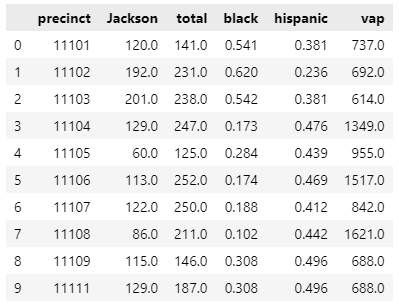
\includegraphics[width=0.6\textwidth]{figures/primary_df.png}
        \caption{Dataframe tập dữ liệu 1}
        \label{fig:primary_df}
    \end{figure}

    Hình \ref{fig:primary_df} thể hiện dataframe của tập dữ liệu 1.

    \begin{figure}[H]
        \centering
        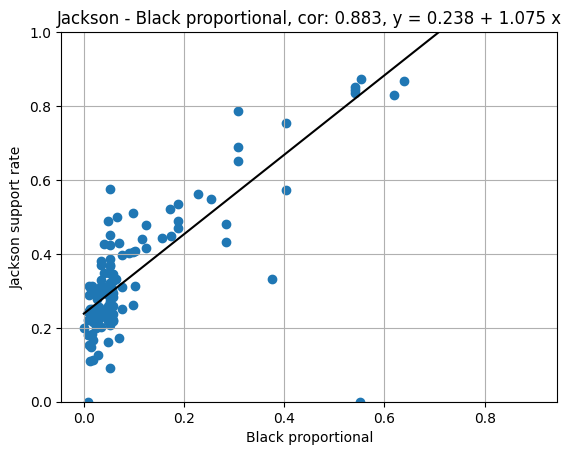
\includegraphics[width=0.6\textwidth]{figures/Jackson_support_rate-Black_proportional-Dataset_1.png}
        \caption{Mối liên hệ giữa tỷ lệ người da đen và tỷ lệ phiếu bầu cho ứng cử viên Jackson}
        \label{fig:Jackson_support_rate_Black_proportional_Dataset_1}
    \end{figure}

    \begin{figure}[H]
        \centering
        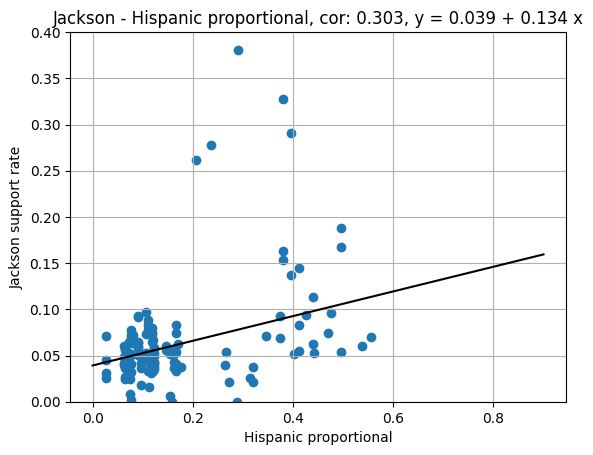
\includegraphics[width=0.6\textwidth]{figures/Jackson_support_rate-Hispanic_proportional-Dataset_1.png}
        \caption{Mối liên hệ giữa tỷ lệ người gốc Tây Ban Nha và tỷ lệ phiếu bầu cho ứng cử viên Jackson}
        \label{fig:Jackson_support_rate_Hispanic_proportional_Dataset_1}
    \end{figure}

    Ta sử dụng mô hình hồi quy tuyến tính để mô hình hóa mối liên hệ giữa tỷ lệ phiếu bầu cho ứng cử viên Jackson tại từng khu vực theo tỷ lệ người da đen hoặc người gốc Tây Ban Nha ở hai hình \ref{fig:Jackson_support_rate_Black_proportional_Dataset_1} và \ref{fig:Jackson_support_rate_Hispanic_proportional_Dataset_1}.
    Khi tỷ lệ người da đen hoặc tỷ lệ người gốc Tây Ban Nha tăng thì tỷ lệ phiếu bầu cho ứng cử viên Jackson cũng tăng nhưng tốc độ tăng là không nhiều.
    Nếu ta giả sử ở một khu vực tỷ lệ người da đen là 100 \% thì tỷ lệ phiếu bầu dự đoán cho ứng cử viên Jackson là $0.035 + 0.31 \times 1=0.3135$.
    Mặt khác, nếu ở một khu vực tỷ lệ người gốc Tây Ban Nha chiếm 100 \% thì tỷ lệ phiếu bầu dự đoán cho ứng cử viên Jackson là $0.039+0.134 \times 1=0.173$.
    Như vậy hai tỷ lệ dự đoán trên vẫn quá thấp để ứng cử viên Jackson có thể thắng cử tại các khu vực này.

    \begin{figure}[H]
        \centering
        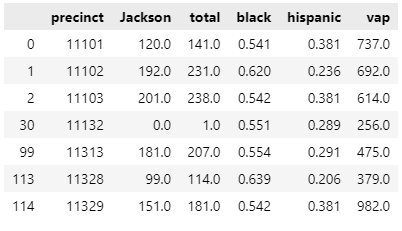
\includegraphics[width=0.6\textwidth]{figures/Predominant_black.png}
        \caption{Những khu vực có người da đen chiếm đa số}
        \label{fig:Predominant_black}
    \end{figure}

    \begin{figure}[H]
        \centering
        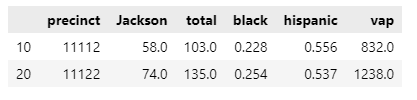
\includegraphics[width=0.6\textwidth]{figures/Predominant_hispanic.png}
        \caption{Những khu vực có người gốc Tây Ban Nha chiếm đa số}
        \label{fig:Predominant_hispanic}
    \end{figure}

    Hình \ref{fig:Predominant_black} và \ref{fig:Predominant_hispanic} lọc ra các khu vực mà người da đen hoặc người gốc Tây Ban Nha chiếm đa số.
    Ở những khu vực có người da đen chiếm đa số chỉ có khu vực 11313 là có tỷ lệ ủng hộ ứng cử viên Jackson khoảng 38 \%, còn lại tất cả các khu vực khác đều có tỷ lệ ủng hộ ứng cử viên Jackson nhỏ hơn 30\%.
    Ở các khu vực có người gốc Tây Ban Nha chiếm đa số thì tỷ lệ ủng hộ ứng cử viên Jackson rất thấp chỉ khoảng 6 - 7\%.

    Như vậy ta thấy từ tập dữ liệu 1, bên nguyên đơn sẽ không thể nào chứng minh được sự cấu thành của điều kiện thứ 2 và điều kiện thứ 3 mà tòa án tối cao đưa ra.
    Tỷ lệ trong nhóm người da đen hoặc người gốc Tây Ban Nha ủng hộ ứng cứ viên Jackson vẫn rất thấp.
    Trong những khu vực người da đen chiếm đa số tỷ lệ người ủng hộ ứng cử viên Jackson không đủ cao hay trong những khu vực người gốc Tây Ban Nha ủng hộ ứng cử viên Jackson lại vô cùng thấp.

    \begin{figure}[H]
        \centering
        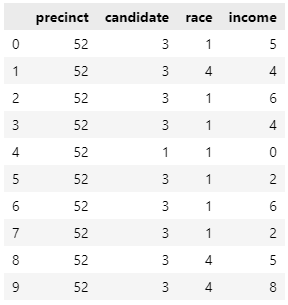
\includegraphics[width=0.6\textwidth]{figures/vote_df.png}
        \caption{Dataframe tập dữ liệu 2}
        \label{fig:vote_df}
    \end{figure}

    Tập dữ liệu thứ 2 gồm các trường khu vực (precinct), ứng cử viên (candidate), chủng tộc (race), mức thu nhập(income).
    Mỗi bản ghi tương ứng với một cử tri tham gia cuộc thăm dò dư luận.
    Để thuận tiện ta sẽ biến đổi dataframe này thành một dataframe khác để thuận tiện cho việc phân tích hơn.
    Ta sẽ tạo một dataframe mới từ dataframe của tập dữ liệu thứ hai bằng cách ứng với mỗi khu vực ta tính mức thu nhập bình quân, tỷ lệ ủng hộ các ứng cử viên và tỷ lệ các nhóm chủng tộc.

    Hình \ref{fig:total_vote_df} hiển thị dataframe mới được tạo ra từ tập dữ liệu thứ 2.
    Ta nhận thấy trong các khu vực, tỷ lệ ủng hộ cho hai ứng cử viên La Rouche và ứng cử viên Gore rất thấp, gần như không ảnh hưởng đến kết quả cuối cùng.
    Ta chỉ xét hai ứng cử viên Jackson và Dukakis có tỷ lệ phiếu bầu đáng kể tại mỗi khu vực.
    Ngoài ra tỷ lệ người châu Á hay các nhóm chủng tộc thiểu số khác không đáng kể nên ta chỉ xét 3 nhóm chủng tộc lớn là người da trắng, người da đen và người gốc Tây Ban Nha
    
    Hình \ref{fig:Jackson_candidate_relationship_factor} và hình \ref{fig:Dukakis_candidate_relationship_factor} thể hiện tỷ lệ ủng hộ của các ứng cử viên theo các yếu tố như mức thu nhập bình quân tại khu vực, tỷ lệ người da trắng, tỷ lệ người da đen, tỷ lệ người gốc Tây Ban Nha trong khu vực đó.
    Với ứng cử viên Jackson, với mức thu nhập bình quân đầu người tăng thì tỷ lệ ủng hộ ứng cử viên Jackson càng giảm.
    Tại các khu vực có tỷ lệ người da đen hoặc người gốc Tây Ban Nha tăng, tỷ lệ ủng hộ ứng cứ viên Jackson tăng rõ rệt.
    Tại các khu vực có tỷ lệ người da trắng tăng, tỷ lệ ủng hộ ứng cử viên Jackson giảm.
    Với ứng cử viên Dukakis thì hoàn toàn trái ngược. Tại các khu vực có thu nhập bình quân đầu người cao, tỷ lệ ủng hộ ứng cử viên Dukakis cũng tăng.
    Tại các nơi có tỷ lệ người da trắng cao, tỷ lệ ủng hộ ứng cử viên Dukakis cũng cao và với tỷ lệ người da đen hoặc người gốc Tây Ban Nha cao thì tỷ lệ ủng hộ ông Dukakis giảm.

    \begin{figure}[H]
        \centering
        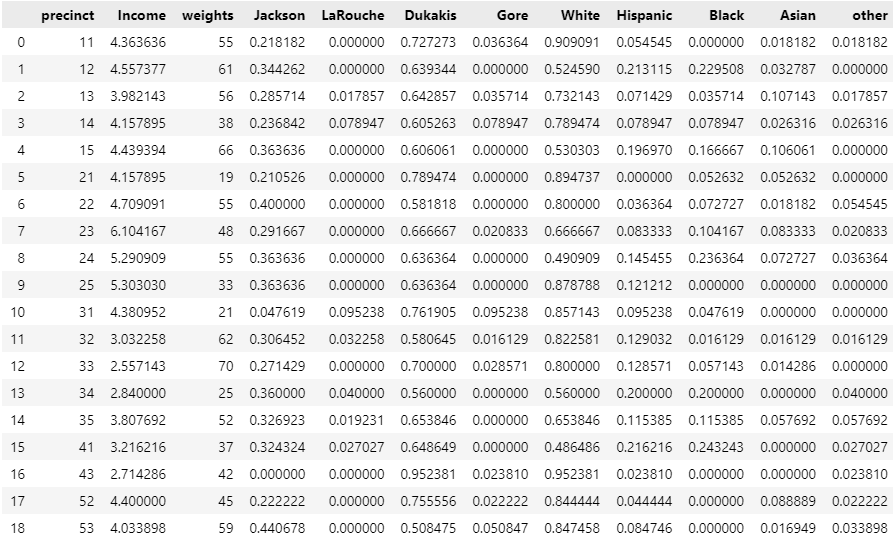
\includegraphics[width=0.9\textwidth]{figures/total_vote_df.png}
        \caption{Dataframe tổng hợp tỷ lệ phiếu bầu của từng ứng cử viên và tỷ lệ từng chủng tộc trong từng khu vực trong cuộc thăm dò ý kiến ở tập dữ liệu 2}
        \label{fig:total_vote_df}
    \end{figure}

    Như vậy theo giả thiết về thu nhập, những người cùng mức thu nhập có chung xu hướng chính trị.
    Nếu ta xem tỷ lệ ủng hộ của một ứng cử viên tại một khu vực là một hàm của mức thu nhập thì ta nhận thấy những khu vực có mức thu nhập càng cao thì tỷ lệ ủng hộ ứng cử viên Jackson càng thấp và đối với ứng cử viên Dukakis thì ngược lại.

    Để xem xét giả thiết về chủng tộc, ta sẽ tính tỷ lệ ủng hộ của các ứng viên trong từng nhóm chủng tộc bằng công thức:

    \begin{equation*}
        \dfrac{\text{số cử tri thuộc chủng tộc X ủng hộ ứng cử viên A}}{\text{số cử tri thuộc chủng tộc X}}
    \end{equation*}

    Ta xây dựng một dataframe mới, gồm các trường là tỷ lệ ủng hộ của từng nhóm chủng tộc cho từng ứng viên ở trong hình \ref{fig:support_rate_df}.
    Hình \ref{fig:support_rate_df} thể hiện dataframe tỷ lệ ủng hộ của từng nhóm chủng tộc cho từng ứng cử viên với định danh "Tên ứng cử viên - Tên nhóm chủng tộc"
    Hình \ref{fig:race_rate_and_candidate_support_rate} biểu diễn mối quan hệ giữa tỷ lệ của từng nhóm chủng tộc và tỷ lệ ủng hộ của ứng cử viên với nhóm chủng tộc đó.
    Đối với nhóm người da đen, tỷ lệ người da đen ủng hộ ứng cử viên Jackson rất cao, ngược lại tỷ lệ ủng hộ ứng cử viên Dukakis nói chung rất thấp.
    Đối với nhóm người da trắng, tỷ lệ người da trắng ủng hộ ứng cử viên Dukakis cao hơn nhiều so với tỷ lệ ủng hộ ứng cử viên Jackson.
    Đối với nhóm người gốc Tây Ban Nha, tỷ lệ ủng hộ ứng cử viên Jackson có xu hướng cao hơn tỷ lệ ủng hộ ứng cử viên Dukakis.
    Như vậy, giả định về chủng tộc đúng với người da đen và người da trắng.
    Khi mà người da đen đa số ủng hộ ứng cử viên Jackson hơn và ngược lại người da trắng đa số ủng hộ ứng cử viên Dukakis.

    \begin{figure}[H]
        \centering
        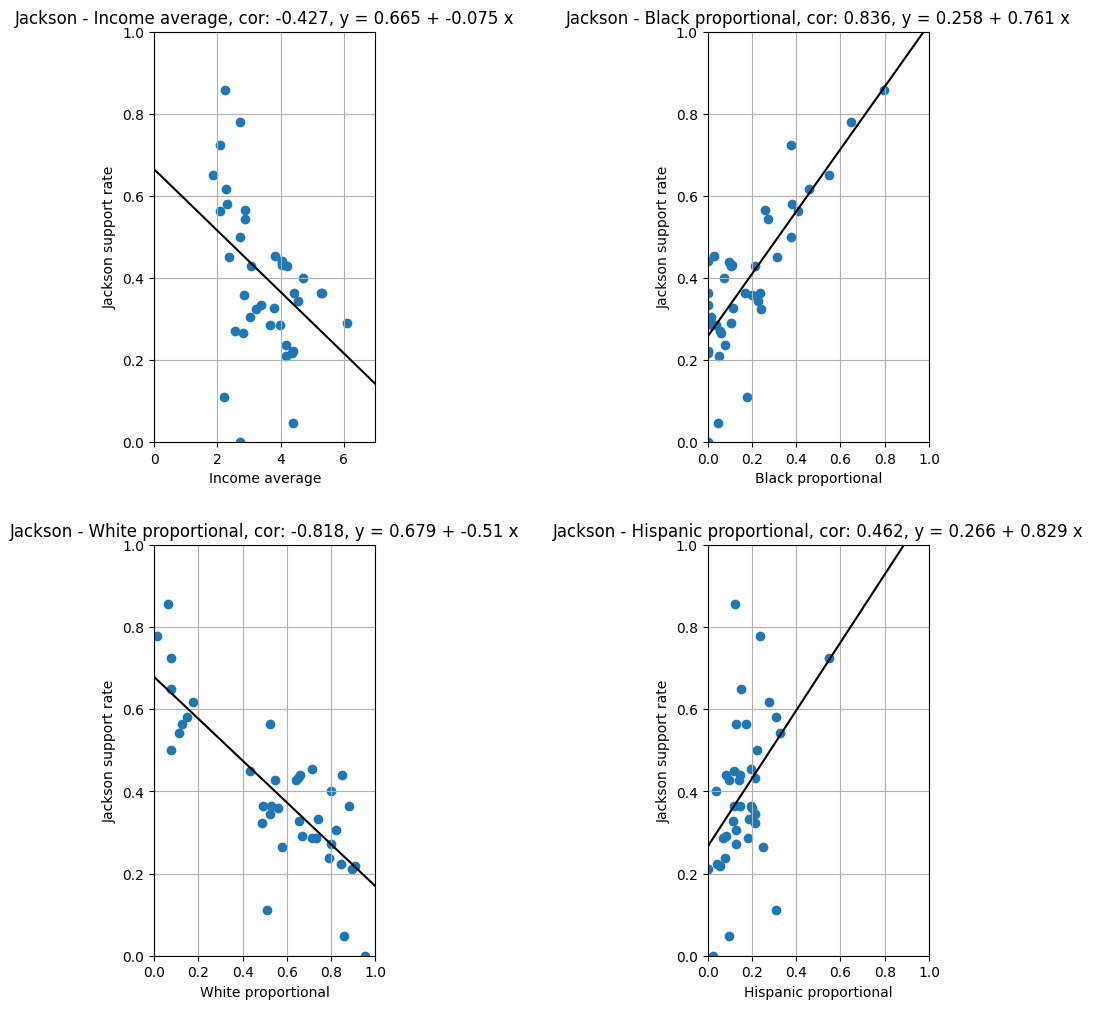
\includegraphics[width=0.9\textwidth]{figures/Jackson_candidate_relationship_factor.png}
        \caption{Mối quan hệ giữa tỷ lệ ủng hộ ứng cử viên Jackson và các yếu tố thu nhập, tỷ lệ người da trắng, tỷ lệ người da đen, tỷ lệ người gốc Tây Ban Nha trong các khu vực ở tập dữ liệu 2}
        \label{fig:Jackson_candidate_relationship_factor}
    \end{figure}

    Một điều khá đáng chú ý nữa từ hình \ref{fig:race_rate_and_candidate_support_rate}, ta nhận thấy tỷ lệ ủng hộ của từng nhóm chủng tộc cho các ứng cử viên trong một khu vực có phụ thuộc vào tỷ lệ của chủng tộc đó trong khu vực đó.
    Cụ thể, ta biết nói chung tỷ lệ ủng hộ ứng cử viên Jackson trong cộng đồng người da đen nói chung là cao nhưng ở một số khu vực có tỷ lệ người da đen thấp thì tỷ lệ ủng hộ ứng cử viên Jackson của người da đen tại khu vực này cũng thấp.
    Điều tương tự cũng xảy ra khi mà tại những khu vực có tỷ lệ người da trắng thấp thì tỷ lệ người da trắng ủng hộ ứng cử viên Jackson cũng cao dù mặt bằng chung tỷ lệ người da trắng ủng hộ ứng cử viên Jackson thấp.
    Điều này ủng hộ cho giả định láng giềng khi những người trong cùng khu vực có xu hướng chọn cùng ứng viên không quan trọng chủng tộc.
    Có thể được giải thích bằng cách những người thuộc nhóm thiểu số ở một khu vực cũng phần nào bị ảnh hưởng xu hướng chính trị bởi nhóm đa số tại khu vực đó.
    Ví dụ, những người da đen là nhóm thiểu số trong một khu vực rất có thể bị ảnh hưởng quan điểm chính trị bởi những người đa trắng là đa số khiến cho tỷ lệ những người da đen tại khu vực này ủng hộ ứng cử viên mà đa số những người da trắng ủng hộ cũng cao và ngược lại.

    Hình \ref{fig:Predominant_black_dataset_2} và hình \ref{fig:Predominant_hispanic_dataset_2} cho biết thông tin tỷ lệ ủng hộ của các chủng tộc đối với các ứng viên mà người da đen (hình \ref{fig:Predominant_black_dataset_2}) chiếm đa số và người gốc Tây Ban Nha chiếm (hình \ref{fig:Predominant_hispanic_dataset_2}) đa số.
    Tại những khu vực người da đen chiếm đa số, tỷ lệ ủng hộ của người da đen đối với ứng cử viên Jackson đều rất cao (> 90\%).
    Tại những khu vực người gốc Tây Ban Nha chiếm đa số, tỷ lệ ủng hộ của người gốc Tây Ban Nha với hai ứng cử viên Jackson và Dukakis là như nhau (50 \% - 50 \%)

    \begin{figure}[H]
        \centering
        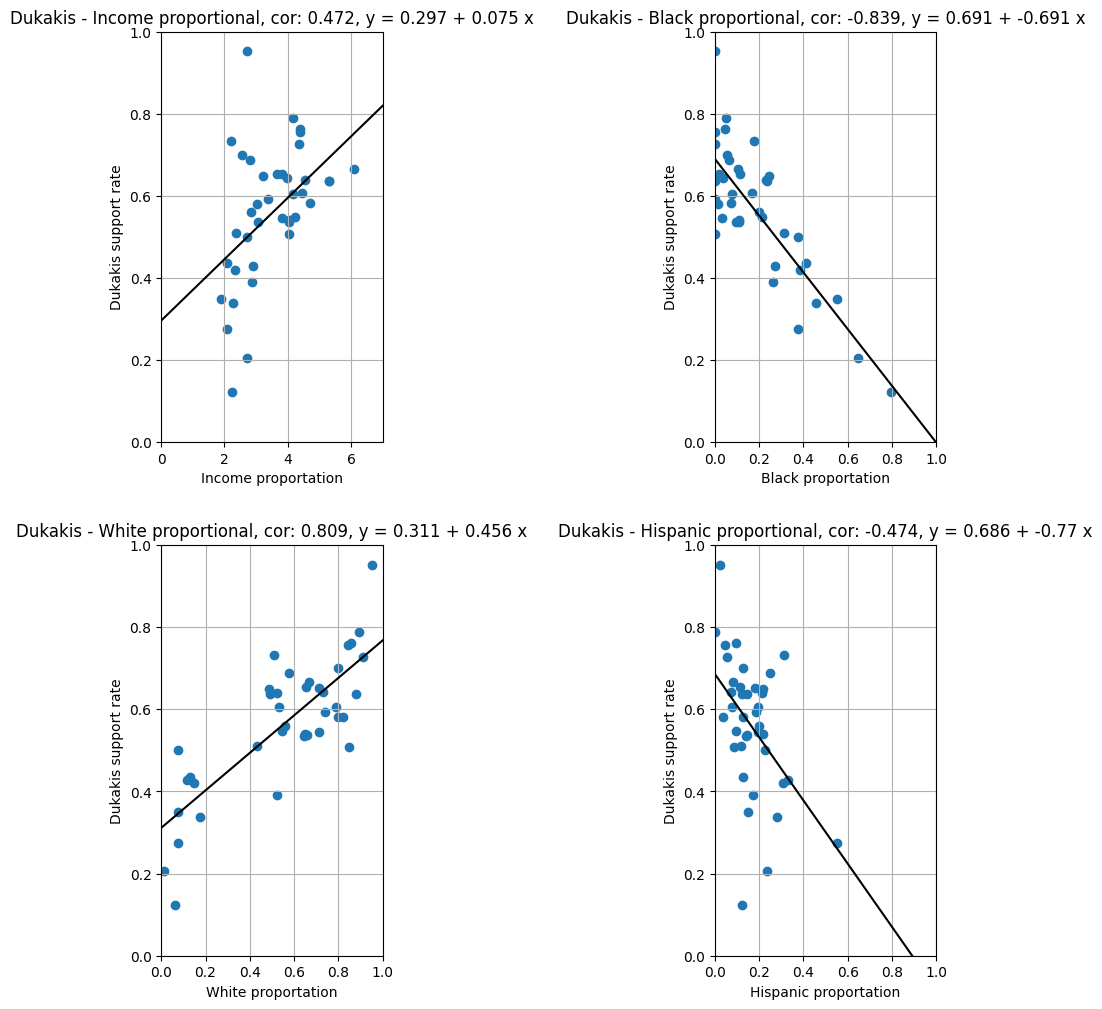
\includegraphics[width=0.9\textwidth]{figures/Dukakis_candidate_relationship_factor.png}
        \caption{Mối quan hệ giữa tỷ lệ ủng hộ ứng cử viên Dukakis và các yếu tố thu nhập, tỷ lệ người da trắng, tỷ lệ người da đen, tỷ lệ người gốc Tây Ban Nha trong các khu vực ở tập dữ liệu 2}
        \label{fig:Dukakis_candidate_relationship_factor}
    \end{figure}


    \begin{figure}[H]
        \centering
        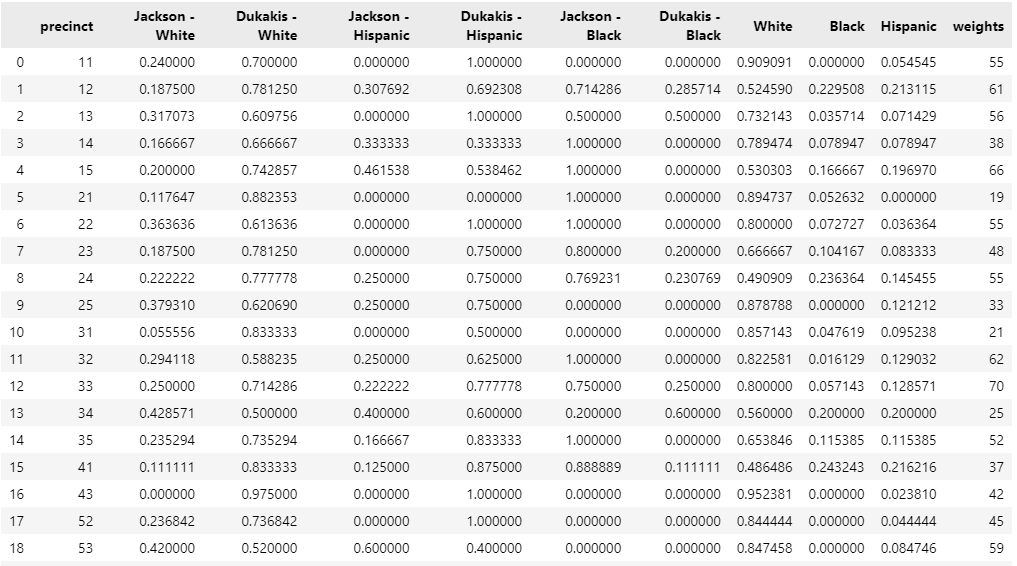
\includegraphics[width=0.9\textwidth]{figures/support_rate_df.png}
        \caption{Dataframe tính tỷ lệ ủng hộ các ứng cử viên Jackson và Dukakis trong từng nhóm chủng tộc trong các khu vực ở tập dữ liệu 2}
        \label{fig:support_rate_df}
    \end{figure}

    \begin{figure}[H]
        \centering
        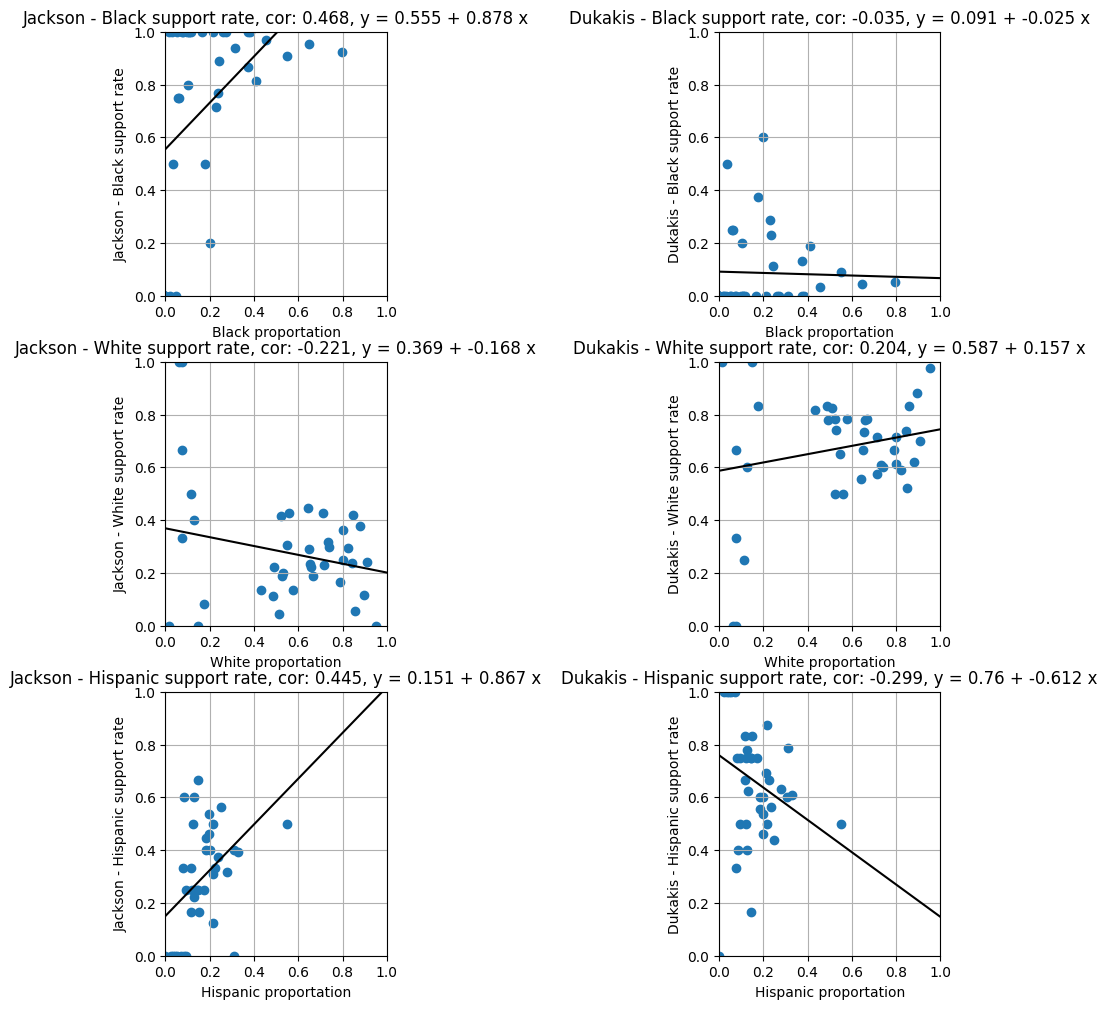
\includegraphics[width=0.9\textwidth]{figures/race_rate_and_candidate_support_rate.png}
        \caption{Tỷ lệ ủng hộ các ứng cử viên Jackson và Dukakis trong từng nhóm chủng tộc trong các khu vực ở tập dữ liệu 2}
        \label{fig:race_rate_and_candidate_support_rate}
    \end{figure}

    \begin{figure}[H]
        \centering
        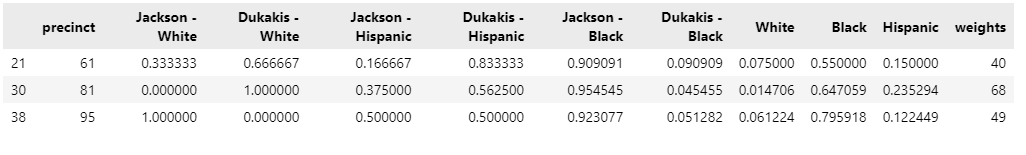
\includegraphics[width=0.8\textwidth]{figures/Predominant_black_dataset_2.png}
        \caption{Những khu vực có người da đen chiếm đa số ở tập dữ liệu 2}
        \label{fig:Predominant_black_dataset_2}
    \end{figure}

    \begin{figure}[H]
        \centering
        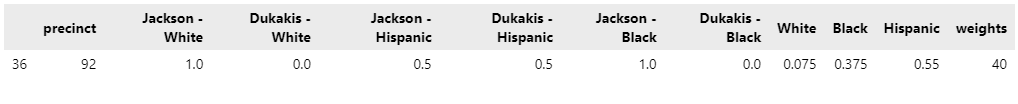
\includegraphics[width=0.8\textwidth]{figures/Predominant_hispanic_dataset_2.png}
        \caption{Những khu vực có người gốc Tây Ban Nha chiếm đa số ở tập dữ liệu 2}
        \label{fig:Predominant_hispanic_dataset_2}
    \end{figure}

    \begin{table}[H]
        \centering
        \begin{tabular}{|c|c|c|}
        \hline
        & Jackson & Dukakis \\
        \hline
        Black & 0.5609 & 0.4391 \\
        \hline
        White & 0.3360 & 0.6640 \\
        \hline
        Hispanic & 0.4645 & 0.5355 \\
        \hline
        \end{tabular}
        \caption{Tỷ lệ ủng hộ tổng quan của các ứng cử viên với từng nhóm chủng tộc}
    \end{table}

    \begin{figure}[H]
        \centering
        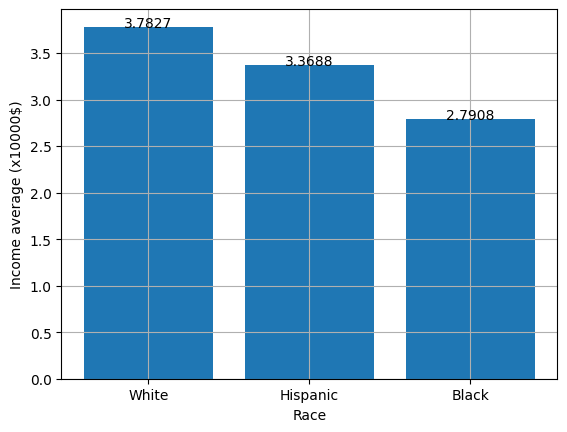
\includegraphics[width=0.5\textwidth]{figures/race_group_income_average.png}
        \caption{Mức thu nhập bình quân theo chủng tộc}
        \label{fig:race_group_income_average}
    \end{figure}
    \end{enumerate}
\end{loigiai}


\newpage
\printbibliography[title={TÀI LIỆU THAM KHẢO}]
\end{document}